% !TEX root = ../LN-Book.tex
%%%%%%%%%%%%%%%%%%%%%%preface.tex%%%%%%%%%%%%%%%%%%%%%%%%%%%%%%%%%%%%%%%%%
% preface
% 2025/03/17 ulgr
%
%%%%%%%%%%%%%%%%%%%%%%%% Springer %%%%%%%%%%%%%%%%%%%%%%%%%%

\preface

\section*{Preface to the Revised First Edition}
	
	When the first edition of these lecture notes appeared in 1986, the theory of one-parameter semigroups of positive operators was undergoing rapid development, stimulated by applications in ergodic theory, evolution equations, stochastics, and mathematical physics. 
	Our goal at the time was to provide a systematic and accessible account of the foundations and structure theory of positive semigroups, with particular emphasis on Banach lattices and \CA-algebras.
	We were gratified by the positive reception the volume received and the extent to which it found use in research and graduate instruction.
	
	Over the past four decades, the mathematical community has continued to draw on the results and techniques developed in these notes. 
	Despite the appearance of newer texts and the evolution of the field, this volume has remained widely cited and used—likely due to its thorough and methodical treatment of a core area in functional analysis. 
	The sustained interest from both researchers and students has encouraged us to prepare this revised first edition.
	
	We have preserved the structure and exposition of the original edition but have made a number of editorial improvements, including transferring the entire book into \LaTeX{}. 
	Obvious misprints have been corrected, references and the subject index have been updated where appropriate, and the notes at the end of each chapter have been expanded to some subsequent developments. 
	However, we have refrained from substantially altering the original content in order to retain the historical character and coherence of the text.
	
	We gratefully acknowledge the efforts of our co-author, Ulrich Groh, who guided the transfer of the manuscript into \LaTeX{}, with the assistance of Klaus-Georg Kuhn and the support of Claude, an artificial intelligence model developed by Anthropic.
	
	It is our hope that this revised edition will continue to serve as a valuable resource for those working in operator theory, functional analysis, and their many applications. 
	We remain deeply grateful to our colleagues and readers who have provided feedback and encouragement over the years.
%% --
%\begin{quote}
%{\itshape
%This second edition of \emph{One-Parameter Semigroups of Positive Operators} is dedicated to the memory 	of our 
%co-authors, Heinrich P.~Lotz (1934--2010) and Ulf Schlotterbeck (1941--2021). 
%Their contributions to the first edition remain an inspiration to us all. 
%We miss their presence and remain grateful for the legacy they have left in this work.}
%\end{quote}
%% --
%\vspace{.75em}
%{\RaggedLeft{The authors} }


%% Please write your preface here

\section*{Preface to the First Edition}

As early as 1948 in the first edition of his fundamental treatise on \emph{Semigroups and Functional Analysis}, E.~Hille expressed the need for 

\begin{quote}
\textit{\ldots developing an adequate theory of transformation semigroups operating in partially ordered spaces} (l.c., Foreword). 
\end{quote}

In the meantime the theory of one-parameter semigroups of positive linear operators has grown continuously. 
Motivated by problems in probability theory and partial differential equations W.~Feller (1952) and R.~S.~Phillips (1962) laid the first cornerstones by characterizing the generators of special positive semigroups. 
In the 60's and 70's the theory of positive operators on ordered Banach spaces was built systematically and is well documented in the monographs of H.~H.~Schaefer (1974) and A.~C.~Zaanen (1983). 
But in this process the original ties with the applications and, in particular, with initial value problems were at times obscured. 
Only in recent years an adequate and up-to-date theory emerged, largely based on the techniques developed for positive operators and thus recombining the functional analytic theory with the investigation of Cauchy problems having positive solutions to each positive initial value. 
Even though this development --- in particular with respect to applications to concrete evolution equations in transport theory, mathematical biology, and physics --- is far from being complete, the present volume is a first attempt to shape the multitude of available results into a coherent theory of one-parameter semigroups of positive linear operators on ordered Banach spaces.

The book is organized as follows.
We concentrate our attention on three subjects of semigroup theory: \emph{characterization}, \emph{spectral theory} and \emph{asymptotic behavior}. 
By \emph{characterization}, we understand the problem of describing special properties of a semigroup, such as positivity, through the generator. 
By \emph{spectral theory} we mean the investigation of the spectrum of a generator. 
\emph{Asymptotic behavior} refers to the orbits of the initial values under a given semigroup and phenomena such as stability.

This program (characterization, spectral theory, asymptotic behavior) is worked out on four different types of underlying spaces.
\newpage
%% --
\begin{enumerate}[label=(\Alph*)]
\item 
On Banach spaces---Here we present the background for the subsequent discussions related to order.

\item 
On spaces $C_{0}(X)$ ($X$ locally compact), which constitute an important class of ordered Banach spaces and where our results can be presented in a form which makes them accessible also for the non-expert in order-theory.

\item 
On Banach lattices, which admit a rich theory and are still sufficiently general as to include many concrete spaces appearing in analysis; e.g., $C_0(X)$, $\mathcal{L}^p(k)$ or $l^p$.

\item 
On non-commutative operator algebras such as \CA- or \WA-algebras, which are not lattice ordered but still possess an interesting order structure of great importance in mathematical physics.

\end{enumerate}
%% --
In each of these cases we start with a short collection of basic results and notations, so that the contents of the book may be visualized in the form of a $4 \times 4$ matrix in a way which will allow \enquote{row readers} (interested in semigroups on certain types of spaces) and \enquote{column readers} (interested in certain aspects) to find a path through the book corresponding to their interest.

We display this matrix, together with the names of the authors contributing to the subjects defined through this scheme.
%% --
%\definecolor{darkgreen}{rgb}{0.0, 0.75, 0.0}
%\begin{table}[ht]
%\centering
%\begin{tabular}{l|c|c|c|c|}
%\cline{2-5}
% & \color{darkgreen}{I} & II & \color{darkgreen}{III} & IV \\
% & \color{darkgreen}{Basic} & Characterization & \color{darkgreen}{Spectral} & Asymptotics \\
% & \color{darkgreen}{Results} &  & \color{darkgreen}{Theory} & \\
%\hline
%\multicolumn{1}{|l|}{A. Banach} & R. Nagel & W. Arendt & G. Greiner & F. Neubrander \\
%\multicolumn{1}{|l|}{Spaces} & U. Schlotterbeck & H. P. Lotz & R. Nagel & \\
%\hline
%\multicolumn{1}{|l|}{B. $C_0(X)$} & R. Nagel & W. Arendt & G. Greiner & A. Grabosch \\
%\multicolumn{1}{|l|}{} & U. Schlotterbeck & & & G. Greiner \\
%\multicolumn{1}{|l|}{} & & & & U. Moustakas \\
%\multicolumn{1}{|l|}{} & & & & F. Neubrander \\
%\hline
%\multicolumn{1}{|l|}{C. Banach} & R. Nagel & G. Arendt & G. Greiner & A. Grabosch \\
%\multicolumn{1}{|l|}{Lattices} & U. Schlotterbeck & & & G. Greiner \\
%\multicolumn{1}{|l|}{} & & & & U. Moustakas \\
%\multicolumn{1}{|l|}{} & & & & R. Nagel \\
%\multicolumn{1}{|l|}{} & & & & F. Neubrander \\
%\hline
%\multicolumn{1}{|l|}{\color{darkgreen}{D. Operator}} & U. Groh & U. Groh & U. Groh & U. Groh \\
%\multicolumn{1}{|l|}{\color{darkgreen}{Algebras}} & & & & \\
%\hline
%\end{tabular}
%\end{table}
%% --
%\definecolor{darkgreen}{rgb}{0.0, 0.75, 0.0}
%\begin{table}[ht]
%\centering
%\begin{tabular}{l|c|c|c|c|}
%\cline{2-5}
% & I & II & III & IV \\
% & Basic & Characterization & Spectral & Asymptotics \\
% & Results &  & Theory & \\
%\hline
%\multicolumn{1}{|>{\columncolor{darkgreen}}l|}{A. Banach} & {R. Nagel} & W. Arendt & G. Greiner & F. Neubrander \\
%\multicolumn{1}{|>{\columncolor{darkgreen}}l|}{Spaces} & U. Schlotterbeck & H. P. Lotz & R. Nagel & \\
%\hline
%\multicolumn{1}{|>{\columncolor{darkgreen}}l|}{B. $C_0(X)$} & R. Nagel & W. Arendt & G. Greiner & A. Grabosch \\
%\multicolumn{1}{|>{\columncolor{darkgreen}}l|}{} & U. Schlotterbeck & & & G. Greiner \\
%\multicolumn{1}{|>{\columncolor{darkgreen}}l|}{} & & & & U. Moustakas \\
%\multicolumn{1}{|>{\columncolor{darkgreen}}l|}{} & & & & F. Neubrander \\
%\hline
%\multicolumn{1}{|>{\columncolor{darkgreen}}l|}{C. Banach} & R. Nagel & G. Arendt & G. Greiner & A. Grabosch \\
%\multicolumn{1}{|>{\columncolor{darkgreen}}l|}{Lattices} & U. Schlotterbeck & & & G. Greiner \\
%\multicolumn{1}{|>{\columncolor{darkgreen}}l|}{} & & & & U. Moustakas \\
%\multicolumn{1}{|>{\columncolor{darkgreen}}l|}{} & & & & R. Nagel \\
%\multicolumn{1}{|>{\columncolor{darkgreen}}l|}{} & & & & F. Neubrander \\
%\hline
%\rowcolor{darkgreen}
%\multicolumn{1}{|l|}{D. Operator} & U. Groh & U. Groh & U. Groh & U. Groh \\
%\rowcolor{darkgreen}
%\multicolumn{1}{|l|}{Algebras} & & & & \\
%\hline
%\end{tabular}
%\end{table}
%%  --

\definecolor{darkgreen}{rgb}{0.0, 0.75, 0.0}

\begin{table}[ht]
\centering
%\begin{tabular}{l|>{\columncolor{darkgreen}}c|c|>{\columncolor{darkgreen}}c|c|}
\begin{tabular}{l|c|c|c|c|}
\cline{2-5}
 & I & II & III & IV \\
 & Basic & Characterization & Spectral & Asymptotics \\
 & Results &  & Theory & \\
\hline
\multicolumn{1}{|l|}{A. Banach} & R. Nagel & W. Arendt & G. Greiner & F. Neubrander \\
\multicolumn{1}{|l|}{Spaces} & U. Schlotterbeck & H. P. Lotz & R. Nagel & \\
\hline
\multicolumn{1}{|l|}{B. $C_0(X)$} & R. Nagel & W. Arendt & G. Greiner & A. Grabosch \\
\multicolumn{1}{|l|}{} & U. Schlotterbeck & & & G. Greiner \\
\multicolumn{1}{|l|}{} & & & & U. Moustakas \\
\multicolumn{1}{|l|}{} & & & & F. Neubrander \\
\hline
\multicolumn{1}{|l|}{C. Banach} & R. Nagel & W. Arendt & G. Greiner & A. Grabosch \\
\multicolumn{1}{|l|}{Lattices} & U. Schlotterbeck & & & G. Greiner \\
\multicolumn{1}{|l|}{} & & & & U. Moustakas \\
\multicolumn{1}{|l|}{} & & & & R. Nagel \\
\multicolumn{1}{|l|}{} & & & & F. Neubrander \\
\hline
%\rowcolor{darkgreen}
\multicolumn{1}{|l|}{D. Operator} & U. Groh & U. Groh & U. Groh & U. Groh \\
%\rowcolor{darkgreen}
\multicolumn{1}{|l|}{Algebras} & & & & \\
\hline
\end{tabular}
\end{table}
%% --
This \enquote{matrix of contents} has been an indispensable guide line in our discussions on the scope and the spirit of the various contributions. 
However, we would not have succeeded in completing this manuscript, as a collection of independent contributions (personally accounted for by the authors), under less favorable conditions than we have actually met. 
For one thing, Rainer Nagel was an unfaltering and undisputed spiritus rector from the very beginning of the project. 
On the other hand we gratefully acknowledge the influence of Helmut H.~Schaefer and his pioneering work on order structures in analysis. 
It was the team spirit produced by this common mathematical background which, with a little help from our friends, made it possible to overcome most difficulties.

We have prepared the manuscript with the aid of a word processor, but we confess that without the assistance of 
Klaus-Georg Kuhn the pitfalls of such a system would have been greater than its benefits.
\vspace{.5cm}
\begin{flushright}\noindent
${}$\hfill {\itshape The authors} \\
\end{flushright}

\vspace{.5cm}
\begin{center}
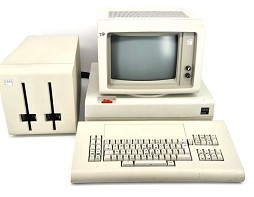
\includegraphics{./part-0/apparaetle.jpg}
\end{center}



